\documentclass[tikz,border=2pt]{standalone}
\begin{document}
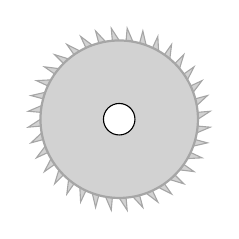
\begin{tikzpicture}
 \fill[gray!35] (0,0) circle (1.0);
 \foreach \i in {1,...,36}{\fill[gray!35] ({360/36*\i}:1.0) -- ({360/36*(\i+0.5)}:1.0) -- ({360/36*(\i+0.5)}:1.16) -- cycle;
  \draw[gray!70] ({360/36*\i}:1.0) -- ({360/36*(\i+0.5)}:1.16) -- ({360/36*(\i+0.5)}:1.0);}
 \draw[gray!70,thick] (0,0) circle (1.0); \fill[white] (0,0) circle (0.2); \draw (0,0) circle (0.2);
\end{tikzpicture}
\end{document}
